\section{Rechtslineare Grammatiken}
\subsection{Rechtslineare Grammatiken}

\begin{frame}{Rechtslineare Grammatiken}
\begin{block}{Def.: Kontextfreie Grammatik}
	Eine \emph{kontextfreie Grammatik} $G$ ist ein Tupel $G = (N,T,S,P)$ mit
	\begin{itemize}
		\item $N$ ist das Alphabet der Nonterminalsymbole, auch Nichtterminalsymbole oder Variablen
		\item $T$ ist das Alphabet der Terminalsymbole, auch Zeichen, mit $N \cap T = \emptyset$
		\item $S$ ist das Startsymbol mit $S \in N$, also die Variable, mit der man beginnt
		\item $P$ ist die Menge der Produktionen mit
			\begin{itemize}
				\item $P \subseteq N \times (N \cup T)^*$, d.h. alle Produktionen besitzen folgende Form:\\
				$V \to w \text{ mit } V \in N \text{ und } w \in (N \cup T)^*$
			\end{itemize}
	\end{itemize}
\end{block}
\end{frame}

\begin{frame}{Rechtslineare Grammatiken}
\begin{block}{Def.: Rechtslineare Grammatik}
	Eine \emph{rechtlineare Grammatik} $G$ ist eine kontextfreie Grammatik $G = (N,T,S,P)$ mit folgenden Einschränkungen für die Produktionen $P$:\\
	\begin{itemize}
			\item $P$ ist entweder von der Form \[
		V \to \omega \text{ mit } \omega \in T^*
	\]
	\item oder \[
		V \to \omega W \text{ mit } \omega \in T^* \text{ und } V,W \in N
	\]
	\item Also: Auf der rechten Seite einer Produktion darf höchstens ein Nonterminalsymbol vorkommen, und wenn dann nur als letztes Symbol.
	\end{itemize}
\end{block}
\pause
\begin{exampleblock}{Beispiel}
	\[
		G = (\set{X,Y}, \set{a,b}, S, \set{X \to aX | bY, Y \to bY | \varepsilon})
	\]
\end{exampleblock}
\end{frame}

\subsection{Reguläre Sprache}
\begin{frame}{Reguläre Sprache}
    \begin{block}{Def.: Reguläre Sprache}
    	Für eine formale Sprache $L$ sind folgende drei Aussagen äquivalent:
    	\begin{itemize}
    		\item $L$ kann von einem endlichen Akzeptor erkannt werden
    		\item $L$ kann durch einen regulären Ausdruck beschrieben werden
    		\item $L$ kann von einer rechtslinearen Grammatik erzeugt werden
    	\end{itemize}
    	Eine solche Sprache $L$ heißt dann auch \emph{reguläre Sprache} (oder Typ-3-Sprache) 
    \end{block}

    \begin{exampleblock}{Aufgabe}
    	Sei $G=(\set{X,Y,Z},\set{a,b},S,P)$ mit $P = \set{
    		X \to aX | bY | \varepsilon,
    		Y \to aX | bZ | \varepsilon, 
    		Z \to aZ | bZ
    	}$.\\ 
    	Zeichne den Akzeptor, der $L(G)$ akzeptiert.\\
    	Wie kann man die Grammatik vereinfachen?
    \end{exampleblock}
\end{frame}

\begin{frame}{Reguläre Sprache}
    \begin{block}{Lösung}
    	\begin{itemize}
    		\item Akzeptor, der $L(G)$ akzeptiert:\\
    		\begin{figure}[ht]
  			\centering
    			\begin{tikzpicture}[shorten >=1pt,node distance=2cm,auto,initial text=,>=stealth]
      				\node[state,initial,accepting]  (q_0)                       {$X$};
	      			\node[state,accepting]          (q_1) [right of= q_0] {$Y$};
	      			\node[state]                    (q_2) [right of= q_1] {$Z$};
	     			\path[->] (q_0) edge [loop below]      node        {$a$} ()
	     			edge [bend right] node [swap] {$b$} (q_1)
	      			(q_1) edge              node        {$b$} (q_2)
	      			edge [bend right] node [swap] {$a$} (q_0)
	      			(q_2) edge [loop below] node        {$a,b$} ()
	      			;
    			\end{tikzpicture}
    		\end{figure}
    		\item Einfacher: $G=(\set{X,Y},\set{a,b},X,P)$ mit $P=\set{X \to a X \mid b Y \mid \varepsilon,\;\; Y \to a X \mid \varepsilon}$
    		\item Oder noch einfacher:
    		$G=(\set{X},\set{a,b},X,P)$ mit $P=\set{X \to a X\mid baX \mid b \mid \varepsilon}$
    	\end{itemize}
    \end{block}
\end{frame}

\subsection{Regex-Bäume}
\begin{frame}{Kantorowitsch-/Regex-Bäume}
    \begin{block}{Def.: Kantorowitsch-/Regex-Baum}
    	Es sei $A$ ein beliebiges Alphabet. Dann heißt ein Baum \emph{Regex-Baum}, falls:
    	\begin{itemize}
    		\item Entweder ist es ein Baum, dessen Wurzel zugleich Blatt ist, und das ist mit einem $x\in A$ oder $\emptyset$ beschriftet,
    		\item oder es ist ein Baum, dessen Wurzel mit $*$ beschriftet ist und die genau einen Nachfolgeknoten hat, der Wurzel eines Regex-Baumes ist
    		\item oder es ist ein Baum, dessen Wurzel mit $\cdot$ oder mit $|$ beschriftet ist und die genau zwei Nachfolgeknoten hat, die Wurzeln zweier Regex-Bäume sind. 
    	\end{itemize}
    \end{block}

    \only<1|handout:1>{
    \begin{exampleblock}{Beispiel}
    	Zeichne den Kantorowitschbaum zum arithmetische Ausdruck
    	\[
    		3+(a+b)*(-c)
    	\]
    \end{exampleblock}
    }

   %  \begin{center}
   %  \begin{tikzpicture}
   %    [level 1/.style={sibling distance=30mm},
   %    level 2/.style={sibling distance=20mm},
   %    level 3/.style={sibling distance=15mm},
   %    nodes={draw,circle,inner sep=0pt, minimum size=7mm},
   %    ->,>=stealth]
      
   %    \node {$+$}
   %    child { node {$3$}  edge from parent  }
   %    child { node {$*$}  edge from parent
   %      % [level 2/.style={sibling distance=15mm}]
   %      child { node {$+$}  edge from parent
   %        % [level 2/.style={sibling distance=15mm}]
   %        child { node {$a$}  edge from parent
   %          % [level 2/.style={sibling distance=15mm}]
   %        }
   %        child { node {$b$}  edge from parent
   %          % [level 2/.style={sibling distance=15mm}]
   %        }
   %      }
   %      child {node {$-$} edge from parent
   %        child { node {$c$}  edge from parent}
   %      }
   %    }
   %    ;
   %  \end{tikzpicture}
  	% \end{center}


    \only<2|handout:2>{
    	\begin{exampleblock}{Aufgabe}
    		Zeichne den Regex-Baum zu folgendem regulären Ausdruck:
    		\[
    			R = ( ( b | \emptyset * ) a ) (b * )
    		\]
    	\end{exampleblock}
    }

    
\end{frame}

\begin{frame}{Kantorowitsch-/Regex-Bäume}
	\begin{block}{Lösung zu $R = ( ( b | \emptyset * ) a ) (b * )$}
		\begin{figure}[ht]
  			\centering
  			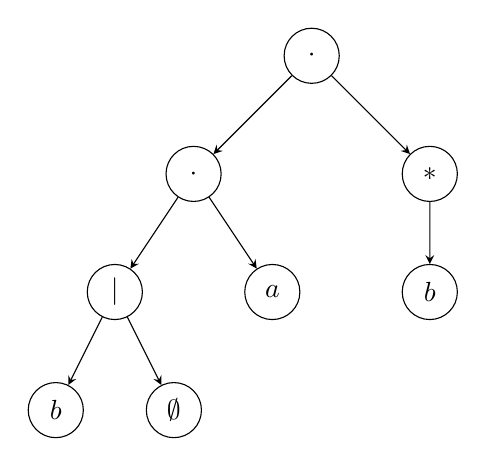
\begin{tikzpicture}
    			[level 1/.style={sibling distance=30mm},
    			level 2/.style={sibling distance=20mm},
    			level 3/.style={sibling distance=15mm},
    			nodes={draw,circle,inner sep=0pt, minimum size=7mm},
    			->,>=stealth]
			    
    			\node {$\cdot$}
    			child { node {$\cdot$}  edge from parent
      			% [level 2/.style={sibling distance=15mm}]
      			child { node {$|$}  edge from parent
        			% [level 2/.style={sibling distance=15mm}]
        			child { node {$b$}  edge from parent
          			% [level 2/.style={sibling distance=15mm}]
        			}
        			child { node {$\emptyset$}  edge from parent
          			% [level 2/.style={sibling distance=15mm}]
        			}
      			}
      			child {node {$a$} edge from parent}
    			}
    			child { node {$*$}  edge from parent
      			% [level 2/.style={sibling distance=15mm}]
      			child { node {$b$}  edge from parent
        			% [level 2/.style={sibling distance=15mm}]
      			}
    			}
    			;
			\end{tikzpicture}
  		\end{figure}
	\end{block}
\end{frame}